\section{Neural Networks and Deep Learning}
This is the first course of deep learning specialization at Coursera taught by Professor Andrew Ng. Here is my certificate after finishing this course (Fig. \ref{C1-Certificate}):

\begin{figure}[!htbp]
    \centering
    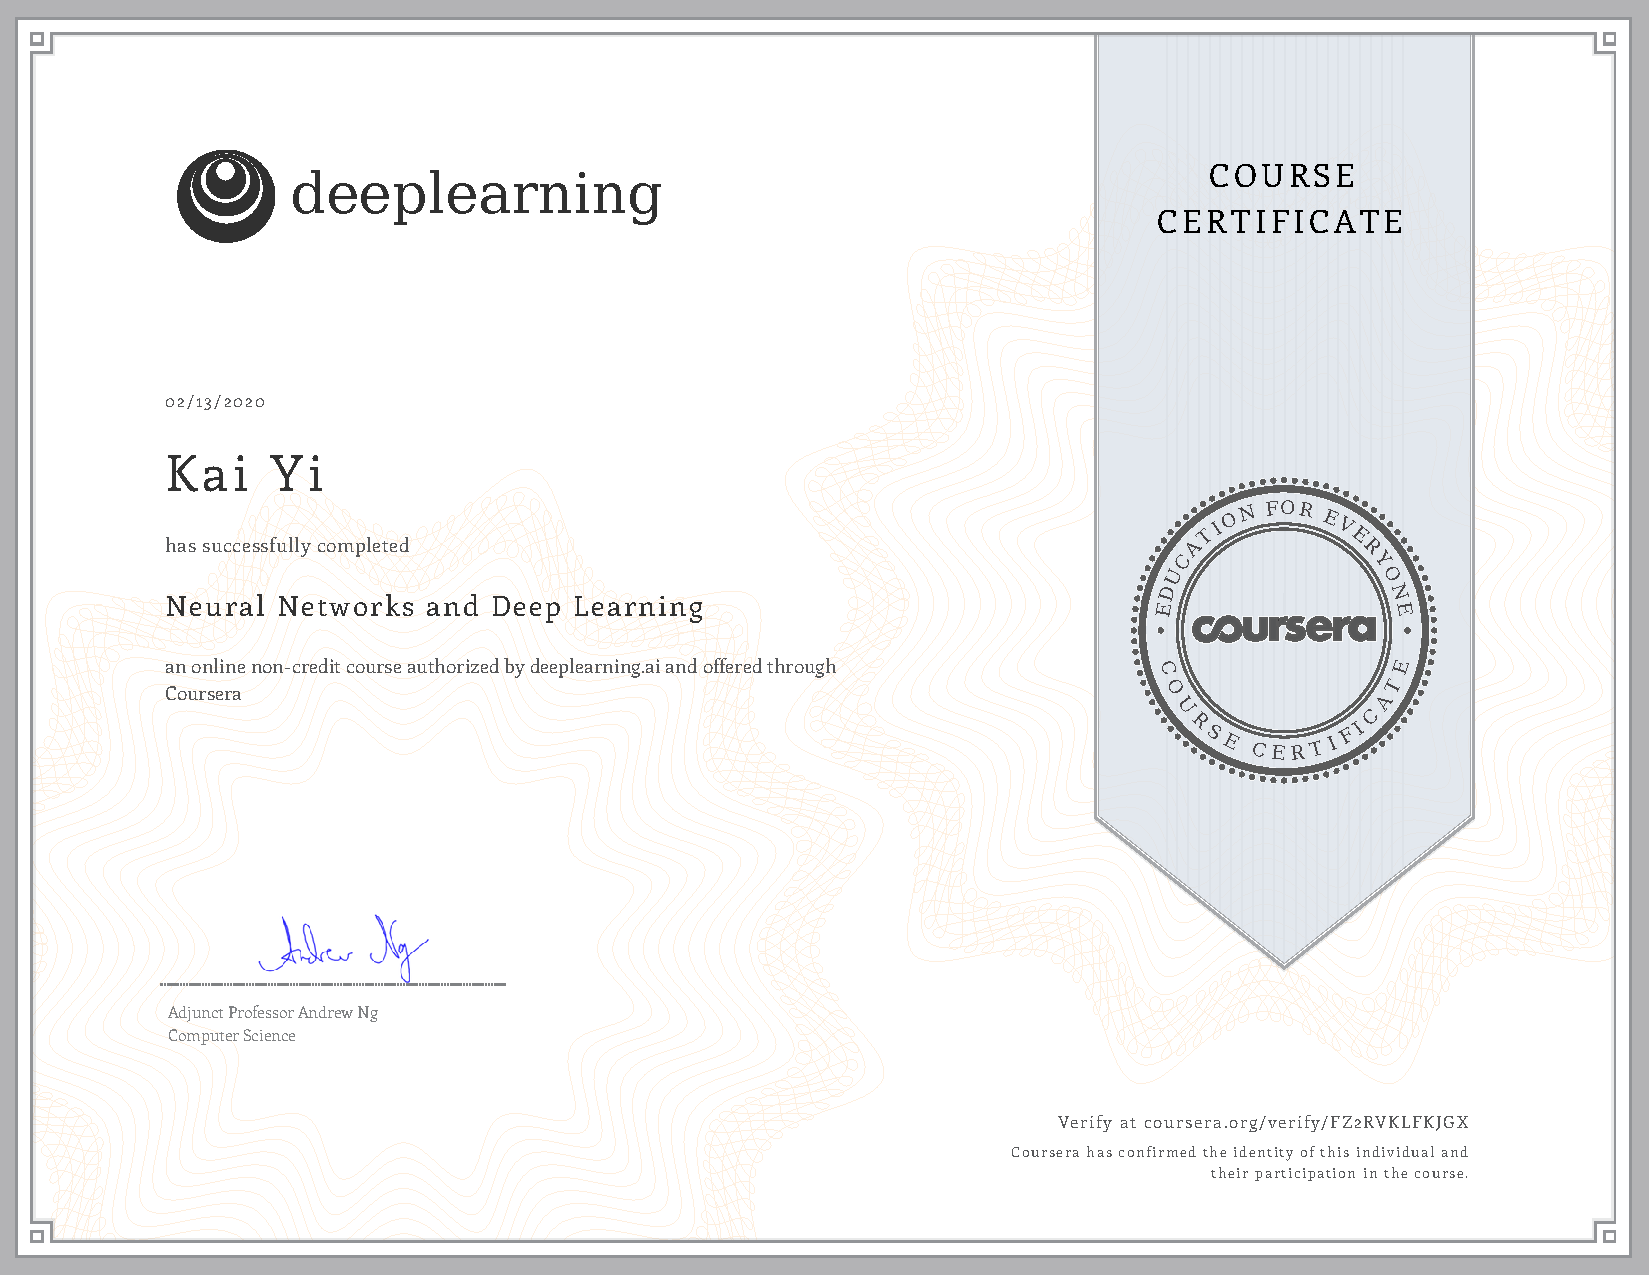
\includegraphics[width=1.0\textwidth]{img/C1-Certificate.pdf}
    \caption{Certificate of Neural Networks and Deep Learning. Obtained in Feb. 2020.}
    \label{C1-Certificate}
\end{figure}

\subsection{Course Overview}
According to the official site of this course, you will learn the foundations of deep learning. When you finish this course, you will:

\begin{itemize}
    \item Understand the major technology trends driving deep learning.
    \item Be able to build, train and apply fully connected deep neural networks.
    \item Know how to implement efficient (vectorized) neural networks.
    \item Understand the key parameters in a neural network's architecture.
\end{itemize}

\subsection{Introduction to Deep Learning}
The section will mainly talk about the major trends driving the rise of deep learning, and understand where and how it is applied today. As I'm very familiar with this part, so I will summarize the background briefly.

Why is deep learning taking off? Data, Computation and Algorithm.

\subsection{Neural Network Basics}
\subsubsection{Logistic Regression}
Algorithm is used for classifications with 2 classes.

$y = w^T x + b$ or $y = sigmoid (w^T x + b)$ if we need y to be in between 0 and 1 (probability).

\subsubsection{Logistic Regression Cost Function}
We don't use square root error ($L(\hat{y}, y) = \frac{1}{2} (\hat{y}- y)^2$) because it leads us to optimization problem which is non=convex, means it contains local optimum points. We are using cross-entropy loss like $L(\hat{y}, y) = - (y\log(\hat{y}) + (1-y)\log(1-\hat{y})$.

To explain the last function lets see:
\begin{itemize}
    \item If $y = 1 \to L(\hat{y},1) = -\log(\hat{y}) \to$ we want $\hat{y}$ to be the largest $\to \hat{y}$ biggest value is 1.
    \item If $y = 0 \to L(\hat{y},0) = -\log(1-\hat{y}) \to$ we want $1-\hat{y}$ to be the largest $\to \hat{y}$ to be smaller as possible because it can only has 1 value.
\end{itemize}

Then the cost function will be: $J(w, b) = \frac{1}{m} \sum(\hat{y}^{(i)}, y^{(i)})$. The cost function is the average of the loss of the entire training set.

\subsubsection{Gradient Descent}
The actual equations we will implement:

\begin{itemize}
    \item $w = w - \alpha dw$ (how much the function slopes in the w direction).
    \item $b = b - \alpha db$ (how much the function slopes in the b direction).
\end{itemize}

$dw$ represents $\frac{dJ(w,b)}{dw}$.

\subsubsection{Logistic Regression Gradient Descent}
In the video, Prof. Andrew discussed the derivatives of gradient descent example for one sample with two features $x1$ and $x2$ (Figure \ref{logistic-regression}).

\begin{figure}[!htbp]
    \centering
    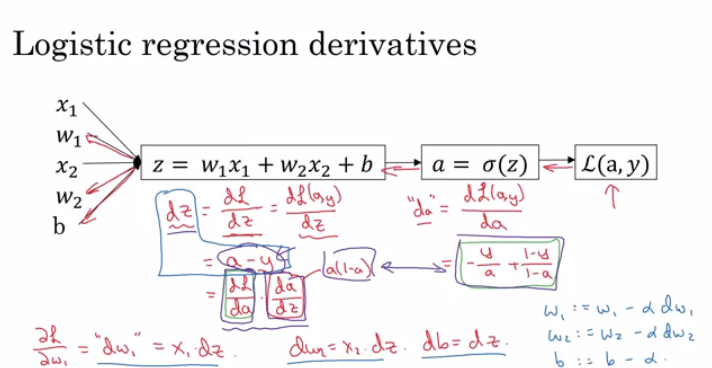
\includegraphics[width=1.0\textwidth, trim={0 0 0 50}, clip]{img/c1/logistic-regression.png}
    \caption{Logistic regression derivatives.}
    \label{logistic-regression}
\end{figure}

\subsubsection{Gradient Descent on m Examples}
The logistic regression pseudo code:

\begin{lstlisting}[language=python]
J = 0; dw1 = 0; dw2 =0; db = 0;     # Devs.
w1 = 0; w2 = 0; b=0;				# Weights
for i = 1 to m
	# Forward pass
	z(i) = W1*x1(i) + W2*x2(i) + b
	a(i) = Sigmoid(z(i))
	J += (Y(i)*log(a(i)) + (1-Y(i))*log(1-a(i)))

	# Backward pass
	dz(i) = a(i) - Y(i)
	dw1 += dz(i) * x1(i)
	dw2 += dz(i) * x2(i)
	db  += dz(i)
J /= m
dw1/= m
dw2/= m
db/= m

# Gradient descent
w1 = w1 - alpha * dw1
w2 = w2 - alpha * dw2
b = b - alpha * db
\end{lstlisting}

The above code should run for some iterations to minimize the error. So there will be two inner loops to implement the logistic regression.

Vectorization is so important on deep learning to reduce loops. In the last code we can make the whole loop in one step using vectorization!

\subsubsection{Vectorization}
Deep learning shines when the dataset are big. However for loops will make you wait a lot for a result. Thats why we need vectorization to get rid of some of our for loops.

NumPy library (dot) function is using vectorization by default. Most of the NumPy library methods are vectorized version.

The vectorization can be done on CPU or GPU thought the SIMD operation. But its faster on GPU.

Whenever possible avoid for loops.

\subsubsection{Vectorizing Logistic Regression}
As an input we have a matrix $X$ and its $[n_x, m]$ and a matrix Y and its $[n_y, m]$.

Thus we have:

\begin{lstlisting}[language=python]
Z = np.dot(W.T,X) + b  # Vectorization, then broadcasting, Z shape is (1, m)
A = 1 / 1 + np.exp(-Z) # Vectorization, A shape is (1, m)
\end{lstlisting}

Vectorizing Logistic Regression's Gradient Output:

\begin{lstlisting}[language=python]
dz = A - Y                  # Vectorization, dz shape is (1, m)
dw = np.dot(X, dz.T) / m    # Vectorization, dw shape is (n_x, 1)
db = dz.sum() / m           # Vectorization, dz shape is (1, 1)
\end{lstlisting}

\subsubsection{Notes on Python and Numpy}
In Numpy, obj.sum(axis = 0) sums the columns while obj.sum(axis = 1) sums the rows.

In Numpy, obj.reshape(1,4) changes the shape of the matrix by broadcasting the values.

Reshape is cheap in calculations so put it everywhere you're not sure about the calculations.

Broadcasting works when you do a matrix operation with matrices that doesn't match for the operation, in this case Numpy automatically makes the shapes ready for the operation by broadcasting the values.

In general principle of broadcasting. If you have an (m,n) matrix and you add(+) or subtract(-) or multiply(*) or divide(/) with a (1,n) matrix, then this will copy it m times into an (m,n) matrix. The same with if you use those operations with a (m , 1) matrix, then this will copy it n times into (m, n) matrix. And then apply the addition, subtraction, and multiplication of division element wise.

Some tricks to eliminate all the strange bugs in the code:

\begin{itemize}
    \item If you didn't specify the shape of a vector, it will take a shape of (m,) and the transpose operation won't work. You have to reshape it to (m, 1).
    \item Try to not use the rank one matrix in ANN.
    \item Don't hesitate to use assert(a.shape == (5,1)) to check if your matrix shape is the required one.
    \item If you've found a rank one matrix try to run reshape on it.
\end{itemize}

Jupyter / IPython notebooks are so useful library in python that makes it easy to integrate code and document at the same time. It runs in the browser and doesn't need an IDE to run.

To open Jupyter Notebook, open the command line and call: jupyter-notebook It should be installed to work.

To Compute the derivative of Sigmoid:
\begin{lstlisting}[language=python]
s = sigmoid(x)
ds = s * (1 - s)       # derivative  using calculus
\end{lstlisting}

To make an image of (width,height,depth) be a vector, use this:

\begin{lstlisting}[language=python]
v = image.reshape(image.shape[0]*image.shape[1]*image.shape[2],1) # reshapes the image.
Gradient descent converges faster after normalization of the input matrices.
\end{lstlisting}

\subsubsection{General Notes}
The main steps for building a Neural Network are:
\begin{itemize}
    \item Define the model structure (such as number of input features and outputs).
    \item Initialize the model's parameters.
    \item Loop. 1) Calculate current loss (forward propagation); 2) Calculate current gradient (backward propagation); 3) Update parameters (gradient descent).
\end{itemize}

Preprocessing the dataset is important.

Tuning the learning rate (which is an example of a "hyperparameter") can make a big difference to the algorithm.

% kaggle.com is a good place for datasets and competitions.


\subsection{Shallow Neural Networks}
In this section, you will learn to build a neural network with one hidden layer, using forward propagation and backpropagation.

\subsubsection{Neural Networks Overview}
In logistic regression we have:

\begin{lstlisting}
X1  \  
X2   ==>  z = WX + b ==> a = Sigmoid(z) ==> L(a,Y)
X3  /
\end{lstlisting}

In neural networks with one layer we will have:

\begin{lstlisting}
X1  \  
X2   =>  z1 = W1X + B1 => a1 = Sigmoid(z1) => z2 = W2a1 + B2 => 
         a2 = Sigmoid(z2) => L(a2,Y)
X3  /
\end{lstlisting}

\subsubsection{Neural Network Representation}
We will define the neural networks that has one hidden layer.

NN contains of input layers, hidden layers, output layers.

Hidden layer means we can't see that layers in the training set.

a0 = x (the input layer)

a1 will represent the activation of the hidden neurons.

a2 will represent the output layer.

We are talking about 2 layers NN. The input layer isn't counted.

\subsubsection{Computing a Neural Network's Output}
Equation of hidden layers (Figure \ref{nn-figure}):

\begin{figure}[!htbp]
    \centering
    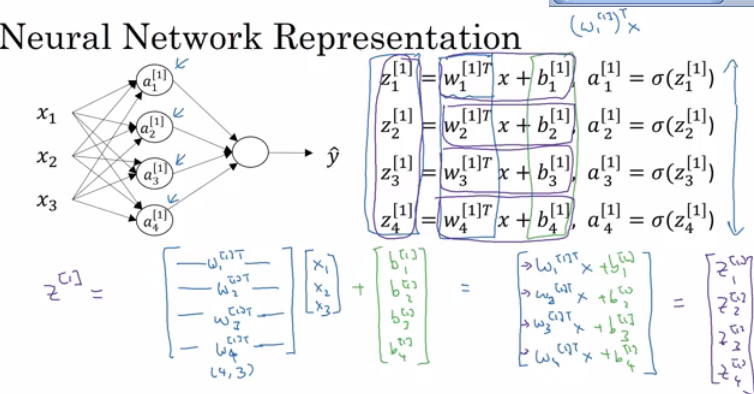
\includegraphics[width=1.0\textwidth, trim={0 0 0 50}, clip]{img/c1/nn-figure.png}
    \caption{Neural Network Representation.}
    \label{nn-figure}
\end{figure}

Shapes of variables:

\begin{itemize}
    \item $w^{[1]}: (n_h, n_x)$, $b^{[1]}: (n_h, 1)$, $z^[1] \to w^{[1]} X + b: (n_h, 1)$, $a^{[1]} \to g(z^{[1]}): (n_h, 1)$.
    \item $w^{[2]}: (1, n_x)$, $b^{[2]}: (1, 1)$, $z^[2] \to w^{[2]} a^{[1]} + b: (1, 1)$, $a^{[2]} \to g(z^{[2]}): (1, 1)$.
\end{itemize}

% Check whether its true.
% Others refer to the assignments for more information.

\subsubsection{Simple Neural Network}
Here is the neural network with a single hidden layer (Figure \ref{classification-kiank}):

\begin{figure}[!htbp]
    \centering 
    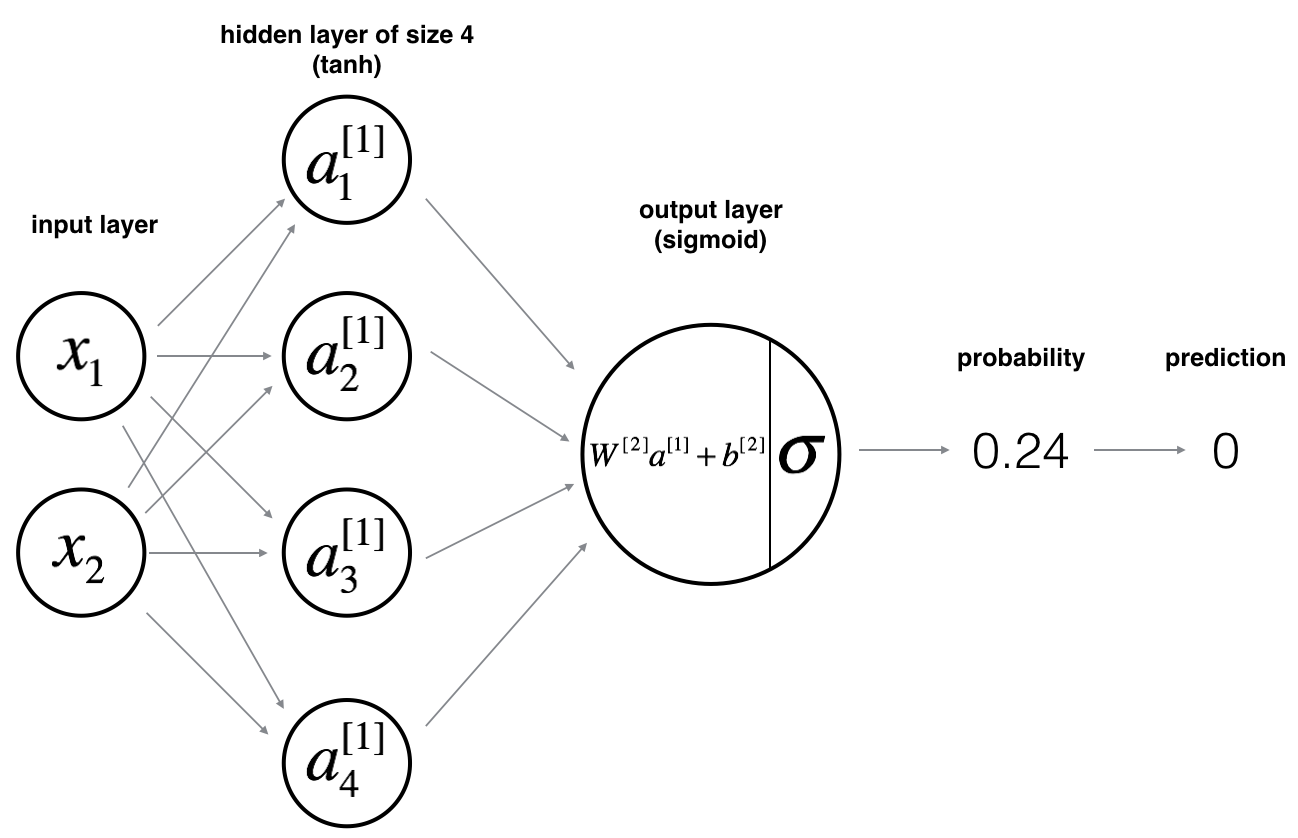
\includegraphics[width=0.8\textwidth, trim={0 0 0 0}, clip]{img/c1/classification_kiank.png}
    \caption{Network architecture with single hidden layer.}
    \label{classification-kiank}
\end{figure}

Mathematically, for one example $x^(i)$, we have: 

\begin{equation}
\centering
\begin{aligned}
z^{[1](i)}&=W^{[1]} x^{(i)}+b^{[1]} \\
a^{[1](i)}&=\tanh \left(z^{[1](i)}\right) \\
z^{[2](i)}&=W^{[2]} a^{[1](i)}+b^{[2]} \\
\hat{y}^{(i)}&=a^{[2](i)}=\sigma\left(z^{[2](i)}\right) \\
y^{(i)}_{\text {prediction}}&=\left\{\begin{array}{ll}
1 & \text { if } a^{[2](i)}>0.5 \\
0 & \text { otherwise }
\end{array}\right.
\end{aligned}
\end{equation}

Given the predictions on all the examples, you can also compute the cost $J$ as follows:

\begin{equation}
    J=-\frac{1}{m} \sum_{i=0}^{m}\left(y^{(i)} \log \left(a^{[2](i)}\right)+\left(1-y^{(i)}\right) \log \left(1-a^{[2](i)}\right)\right)
\end{equation}

The general methodology to build a neural network is to:

\begin{itemize}
    \item[i.]  Define the neural network structure (number of input units, number of hidden units, etc).
    \item[ii.] Initialize the model's parameters.
    \item[iii.] Loop: 1) Implement forward propagation; 2) Compute loss; 3) Implement backward propagation to get the gradients; 4) Update parameters (gradient descent).
\end{itemize}

\subsubsection{Gradient of NN with One Hidden Unit}
Here is the updating rules for the neural network with one hidden unit (Figure \ref{grad-summary}):

\begin{figure}[!htbp]
    \centering 
    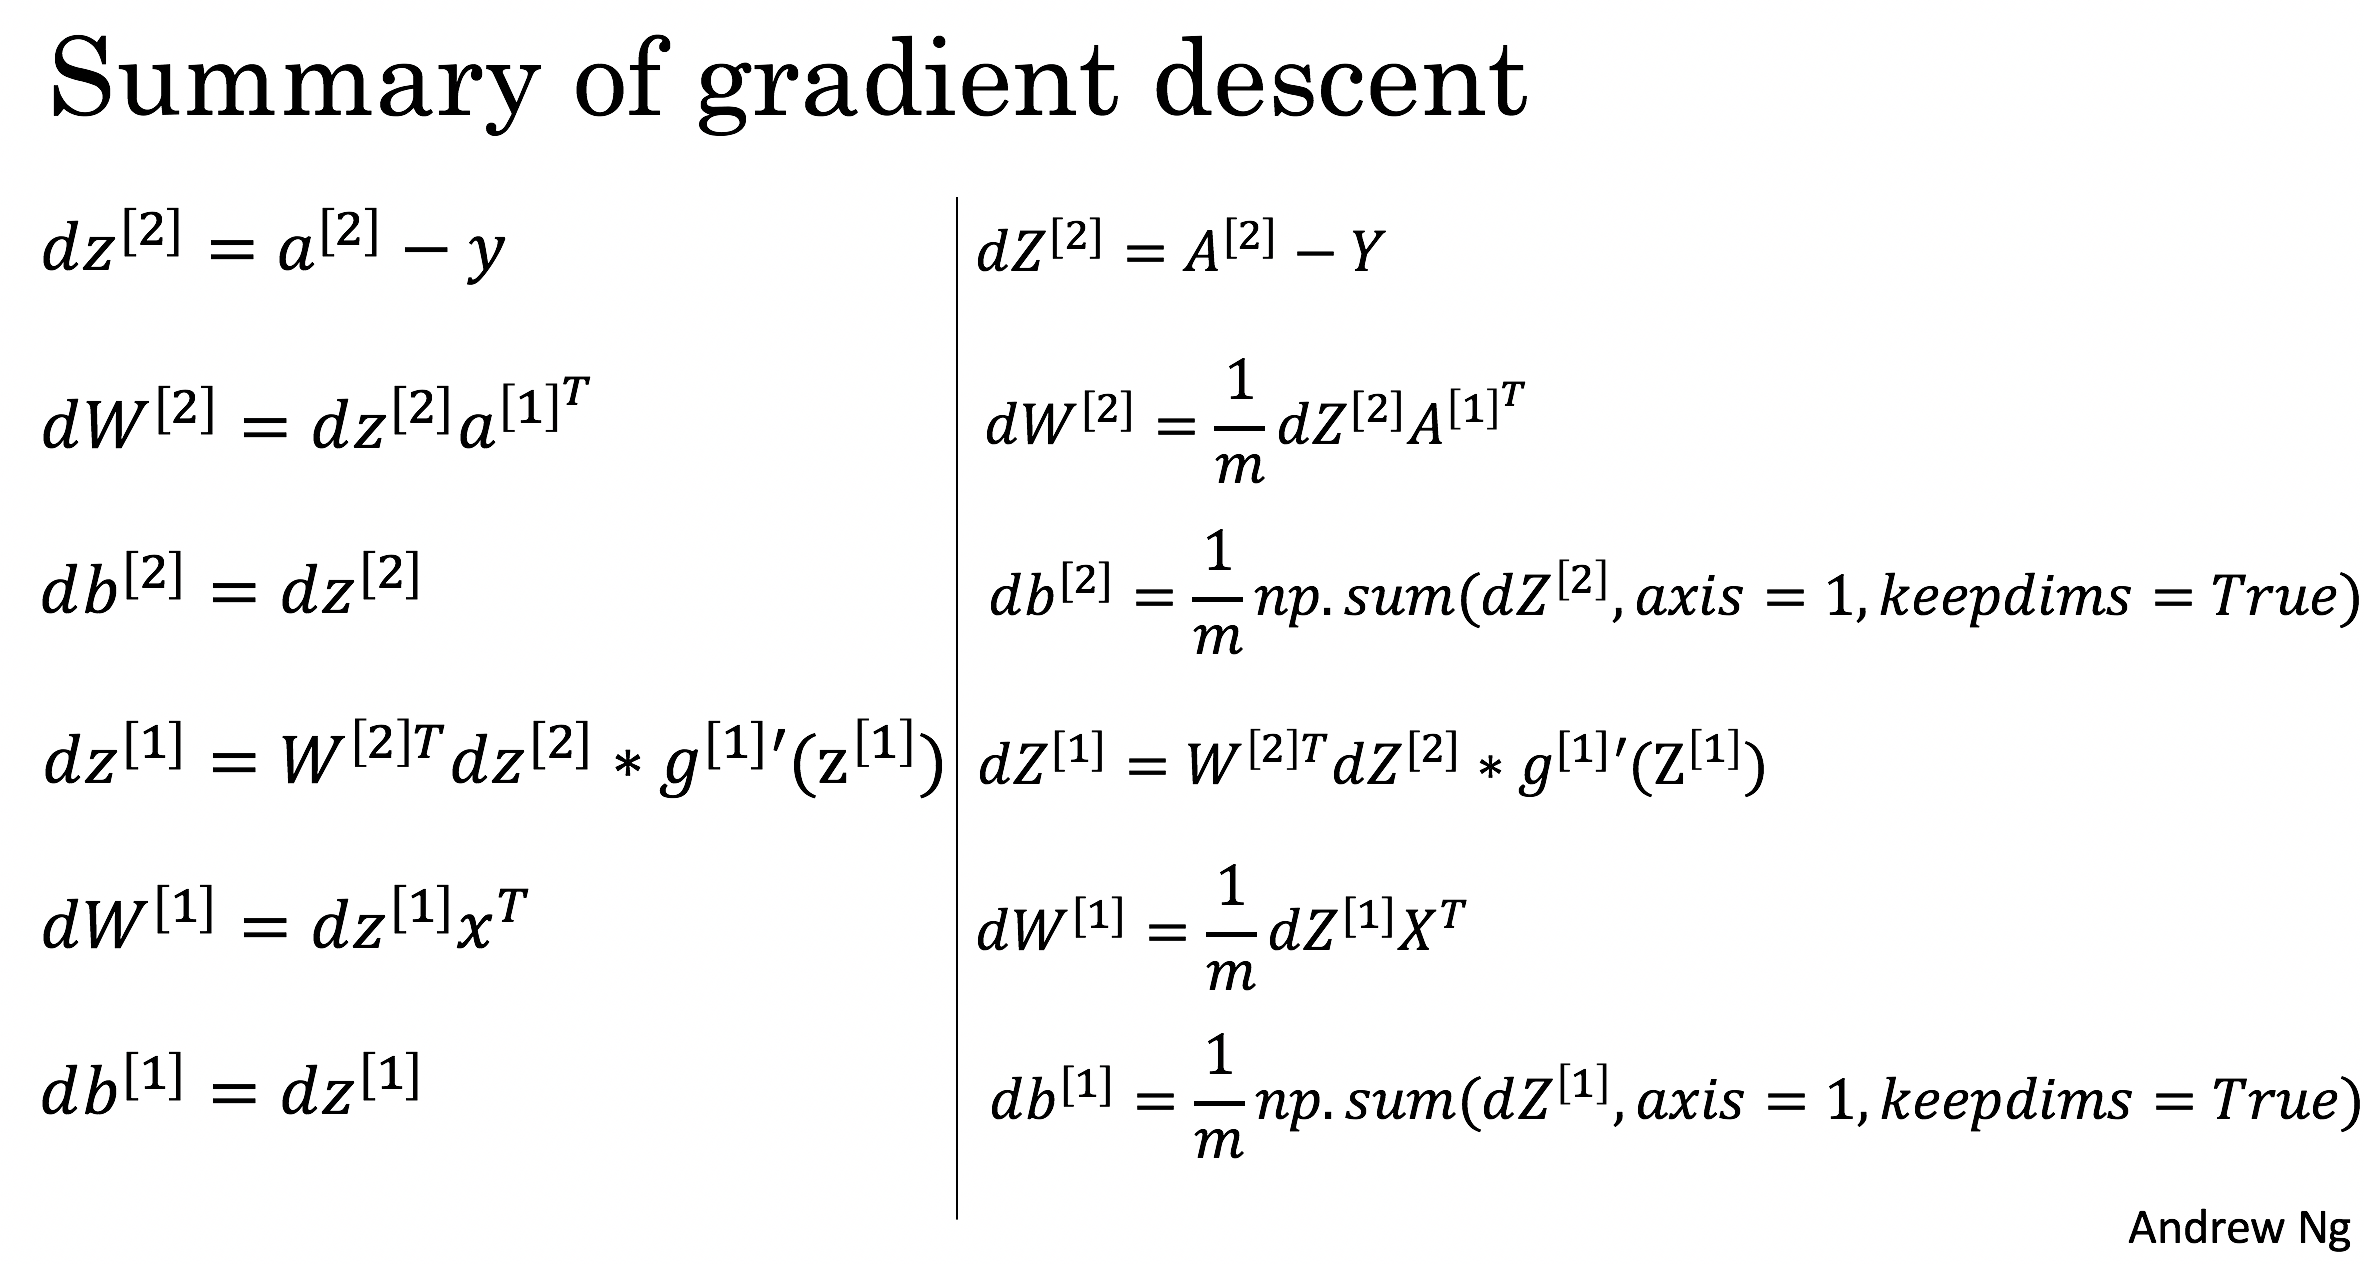
\includegraphics[width=1.0\textwidth, trim={0 0 0 60}, clip]{img/c1/grad_summary.png}
    \caption{Summary of gradient descent.}
    \label{grad-summary}
\end{figure}


\subsection{Deeper Neural Networks}
As the pipeline for deeper neural network is very similar to shallow neural network, so I will summarize this part briefly.

\subsubsection{Building Your Deeper Neural Network: Step by Step}
The pipeline of parameters updating (Figure \ref{final-outline}):

\begin{figure}[!htbp]
    \centering 
    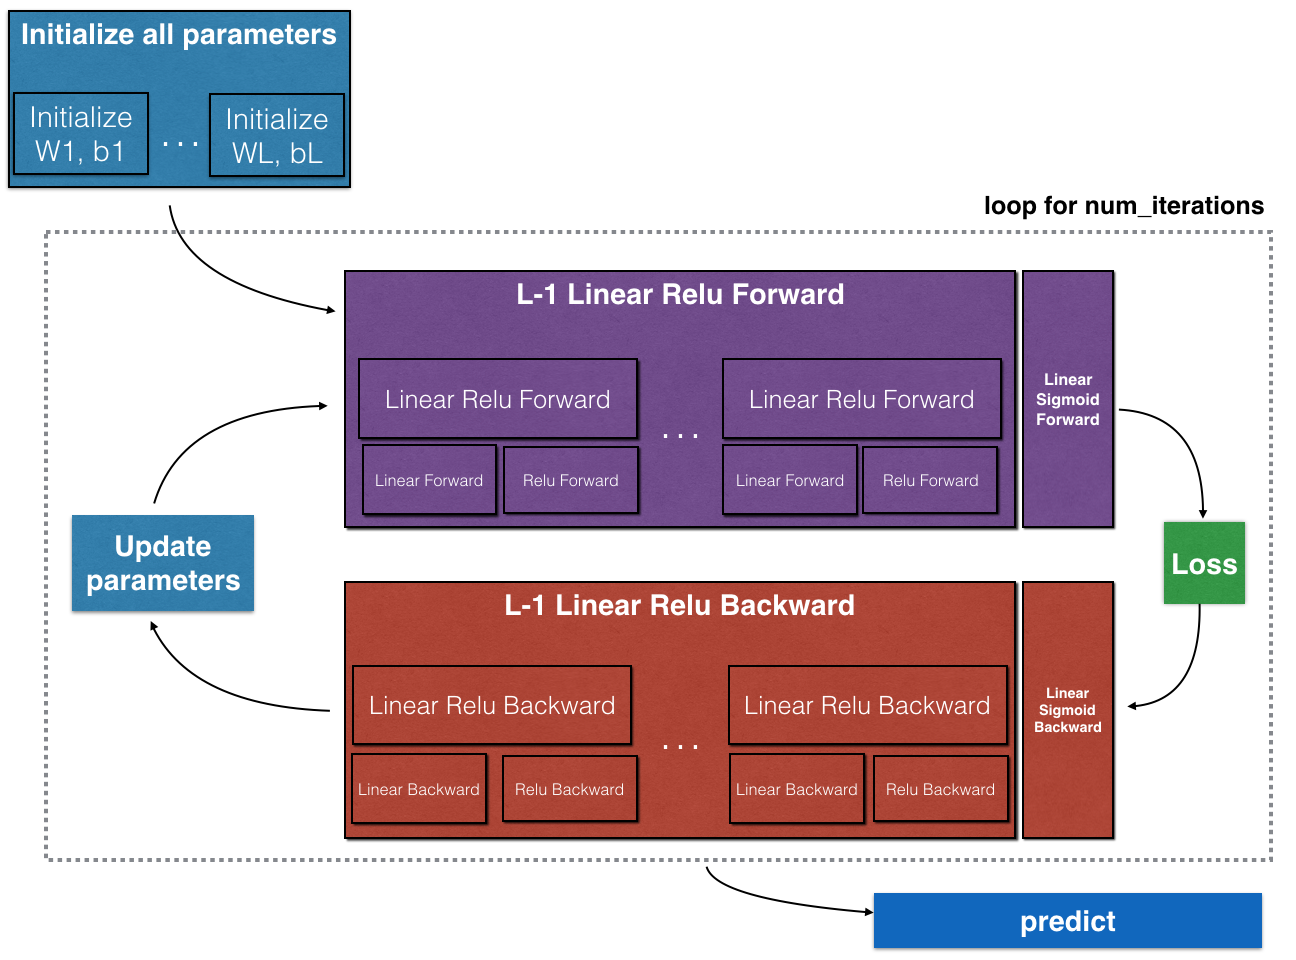
\includegraphics[width=1.0\textwidth, trim={0 0 0 0}, clip]{img/c1/final outline.png}
    \caption{The pipeline of parameters updating.}
    \label{final-outline}
\end{figure}

\paragraph{Forward Propagation}
The linear forward module (vectorized over all the examples) computes the following equations:

\begin{equation}
    Z^{[l]} = W^{[l]}A^{[l-1]} + b^{[l]}
\end{equation}

where $A^{[0]} = X$.

\paragraph{Cost Function}
\begin{equation}
    -\frac{1}{m} \sum_{i=1}^{m}\left(y^{(i)} \log \left(a^{[L](i)}\right)+\left(1-y^{(i)}\right) \log \left(1-a^{[L](i)}\right)\right)
\end{equation}

\paragraph{Illustrations of forward and backward propagation} Could refer to Figure \ref{backprop-kiank}.

\begin{figure}[!htbp]
    \centering 
    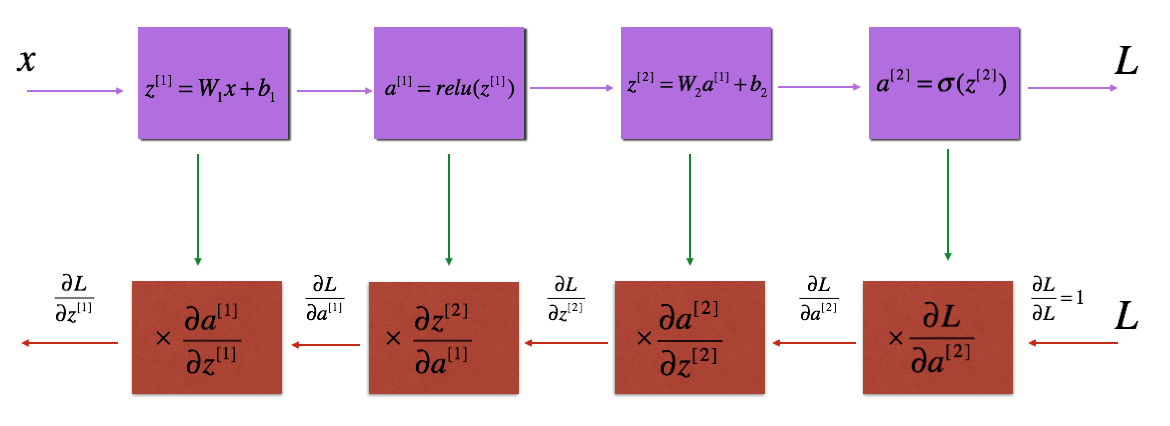
\includegraphics[width=1.0\textwidth, trim={0 0 0 0}, clip]{img/c1/backprop_kiank.png}
    \caption{Forward and Backward propagation for LINEAR->RELU->LINEAR->SIGMOID. The purple blocks represent the forward propagation, and the red blocks represent the backward propagation.}
    \label{backprop-kiank}
\end{figure}

\paragraph{Backward Gradients}
Here are the gradients for layer $l$:
\begin{equation}
\begin{aligned}
d W^{[l]} &=\frac{\partial \mathcal{J}}{\partial W^{[l]}}=\frac{1}{m} d Z^{[l]} A^{[l-1] T} \\
d b^{[l]} &=\frac{\partial \mathcal{J}}{\partial b^{[l]}}=\frac{1}{m} \sum_{i=1}^{m} d Z^{[l](i)} \\
d A^{[l-1]} &=\frac{\partial \mathcal{L}}{\partial A^{[l-1]}}=W^{[l] T} d Z^{[l]}
\end{aligned}
\end{equation}

\paragraph{Update Parameters}:

\begin{equation}
W^{[l]}=W^{[l]}-\alpha d W^{[l]} \\
b^{[l]}=b^{[l]}-\alpha d b^{[l]} \\
\end{equation}



\newpage